\chapter{Experiments}
As mentioned in the previous chapter, the process of finding was an iterative one of running an experiment, analyzing the generated data, draw conclusions and then repeat the steps with a new experiments designed to amend the mistakes of the previous experiment. This chapter will go through each of these steps and explain the insights that were gained.

This chapter presents the flow of analysis as it was carried out, rather 

A summary and discussion of the results is found in chapter \ref{chapter:discussion}.


\section{D3}
In this experiment, the number of \ssmmnAgents and \scnAgents as well all the latency parameters were included in the individuals. The genetic algorithm was run for 1000 generations with a population size of 200. A total of 


This data set was generated by including all the model parameters concerning time latency as well as the number of agents into the individuals in the genetic algorithm. Due to the high number of variables, the data turned out to be difficult to analyze, as too many factors pertaining to the simultaneous change of several parameters influenced the fitness values. Thus, not many definitive results concerning the impact of time latency of market behavior were derived from this data set. The reason why it is still included in the thesis is that the data did provide hints on how to proceed with the analysis of the model. Furthermore, the data set proved useful for developing the tools used to analyze the data sets that were generated later, and hence this section is intended to illustrate the motivation for applying these tools.

Scatter plots of the fitness data before and after preprocessing were already shown in figure \ref{figure:scatter_log_transform}.

\begin{table}
	\centering
	\begin{tabular}{l|l}
	Dataset id & Parameters in genes\\
	\dthree & \sclatencymu, \sclatencys, \scnAgents, \scthinkmu, \scthinks, \sctimehorizonmu, \sctimehorizons, \scwaitTimeBetweenTradingmu, \scwaitTimeBetweenTradings, \ssmmlatencymu, \ssmmlatencys, \ssmmnAgents, \ssmmthinkmu, \ssmmthinks	
	\end{tabular}
\end{table}

Free parameters:

Data set \dthree was the first run of the genetic algorithm that actually produced something that looked like results. The following parameters were included in the genetic algorithm individuals:
\begin{center}
\sclatencymu, \sclatencys, \scnAgents, \scthinkmu, \scthinks, \sctimehorizonmu, \sctimehorizons, \scwaitTimeBetweenTradingmu, \scwaitTimeBetweenTradings, \ssmmlatencymu, \ssmmlatencys, \ssmmnAgents, \ssmmthinkmu, \ssmmthinks
\end{center}

Fixed parameters:




\begin{figure}
	%issue 15
	\centering
	\subcaptionbox{Evolution of \ssmmlatencymu and \sclatencymu}
	[0.49\linewidth]{\includegraphics[width=0.5\textwidth]{82_generation_plots/d3/latpars_mu.png}}
	\subcaptionbox{Evolution of \ssmmthinkmu and \scthinkmu}
	[0.49\linewidth]{\includegraphics[width=0.5\textwidth]{82_generation_plots/d3/thinkpars_mu.png}}
	\subcaptionbox{Evolution of \nmm and \nsc}
	[0.49\linewidth]{\includegraphics[width=0.5\textwidth]{82_generation_plots/d3/nAgents.png}}	\caption{Evolution of time delay parameters common both HFT agent types, and of the number of agents in experiment \dthree}\label{fig:d3_evolution_latpars_nAgents}
\end{figure}


\begin{figure}
	%issue 15
	\subcaptionbox{Evolution of \sctimehorizonmu}
	[0.49\linewidth]{\includegraphics[width=0.5\textwidth]{82_generation_plots/d3/sctimehorizon_mu.png}}
	\subcaptionbox{Evolution of \scwaitTimeBetweenTradingmu}
	[0.49\linewidth]{\includegraphics[width=0.5\textwidth]{82_generation_plots/d3/scwaittime_mu.png}}
	\caption{Evolution of chartist-specific strategy parameters in experiment \dthree}\label{fig:d3_evolution_thinkpars}
\end{figure}

\begin{figure}
	%issue 15
	\centering
	\subcaptionbox{Evolution of \roundstable}
	[0.49\linewidth]{\includegraphics[width=0.5\textwidth]{82_generation_plots/d3/round_stable.png}}
	\subcaptionbox{Evolution of \timetoreachnewfundamental}
	[0.49\linewidth]{\includegraphics[width=0.5\textwidth]{82_generation_plots/d3/time_to_reach_new_fundamental.png}}
	\subcaptionbox{Evolution of \stdev}
	[0.49\linewidth]{\includegraphics[width=0.5\textwidth]{82_generation_plots/d3/stdev.png}}
	\subcaptionbox{Evolution of \overshoot}
	[0.49\linewidth]{\includegraphics[width=0.5\textwidth]{82_generation_plots/d3/overshoot.png}}
	\caption{Evolution of the four fitness measures in experiment \dthree}\label{fig:d3_evolution_fitness}
\end{figure}


EVEN THOUGH ROUND STABLE AND TIME TO REACH NEW FUNDAMENTAL SEEM SIMILAR, THEY ARE NOT CORRELATED SO MUCH. WRITE ABOUT WHAT THIS MEANS (e.g. some markets reach new fundamental quickly, but never become stable, etc.)

\subsection{Section summary}
In summary, the main problem with this data set was that it contained mostly simulations with few or no high frequency traders. 

\section{D9: Fixing the number of high frequency traders}

\subsection{Parameter and fitness evolution}

\begin{figure}
	%issue 15
	\centering
	\subcaptionbox{Evolution of \ssmmlatencymu and \sclatencymu}
	[0.49\linewidth]{\includegraphics[width=0.5\textwidth]{82_generation_plots/d9/latpars_mu.png}}
	\subcaptionbox{Evolution of \ssmmthinkmu and \scthinkmu}
	[0.49\linewidth]{\includegraphics[width=0.5\textwidth]{82_generation_plots/d9/thinkpars_mu.png}}
	\caption{Evolution of time delay parameters common both HFT agent types in experiment \dthree}
	\label{fig:d9_evolution_latpars}
\end{figure}


\begin{figure}
	%issue 15
	\subcaptionbox{Evolution of \sctimehorizonmu}
	[0.49\linewidth]{\includegraphics[width=0.5\textwidth]{82_generation_plots/d9/sctimehorizon_mu.png}}
	\subcaptionbox{Evolution of \scwaitTimeBetweenTradingmu}
	[0.49\linewidth]{\includegraphics[width=0.5\textwidth]{82_generation_plots/d9/scwaittime_mu.png}}
	\caption{Evolution of chartist-specific strategy parameters in experiment \dnine}
	\label{fig:d9_evolution_thinkpars}
\end{figure}



\begin{figure}
	%issue 15
	\centering
	\subcaptionbox{Evolution of \roundstable}
	[0.49\linewidth]{\includegraphics[width=0.5\textwidth]{82_generation_plots/d9/round_stable.png}}
	\subcaptionbox{Evolution of \timetoreachnewfundamental}
	[0.49\linewidth]{\includegraphics[width=0.5\textwidth]{82_generation_plots/d9/time_to_reach_new_fundamental.png}}
	\subcaptionbox{Evolution of \stdev}
	[0.49\linewidth]{\includegraphics[width=0.5\textwidth]{82_generation_plots/d9/stdev.png}}
	\subcaptionbox{Evolution of \overshoot}
	[0.49\linewidth]{\includegraphics[width=0.5\textwidth]{82_generation_plots/d9/overshoot.png}}
	\caption{Evolution of the four fitness measures in experiment \dnine}
	\label{fig:d9_evolution_fitness}
\end{figure}

\subsection{Visualizing the data set}
\begin{figure}
\centering
\subcaptionbox{$\log \stdev$ vs. $\log \roundstable$ vs. \timetoreachnewfundamental}
[0.49\linewidth]{\includegraphics[width=0.5\textwidth]{21_scatter_plots/d9/d.png}}
\subcaptionbox{\roundstable vs. \timetoreachnewfundamental vs. \stdev}
[0.49\linewidth]{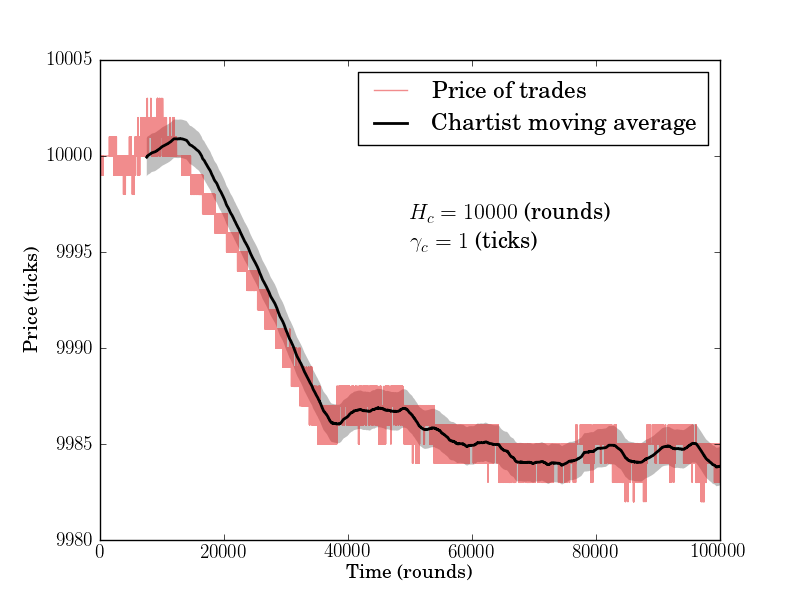
\includegraphics[width=0.5\textwidth]{21_scatter_plots/d9/c.png}}
\subcaptionbox{$\log \overshoot$ vs . $\log \stdev$ vs. \timetoreachnewfundamental}
[0.49\linewidth]{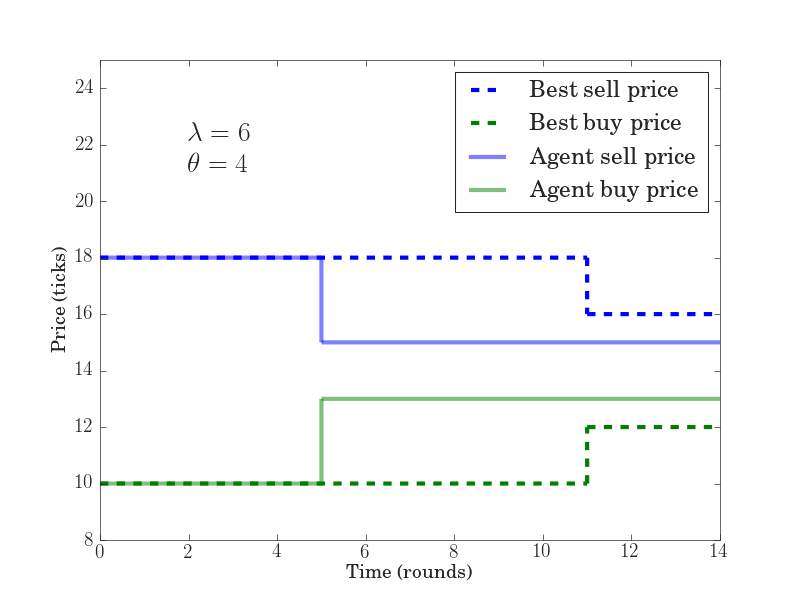
\includegraphics[width=0.5\textwidth]{21_scatter_plots/d9/b.png}}
\caption{Scatter plots of fitness measures in experiment \dnine. }
\label{figure:d9_scatter_fitness}
\end{figure}

Scatter plots are probably among the most rudimentary of techniques for data analysis, yet they can be incredibly informative, especially when the data that is visualized is low-dimensional.
The two plots in figure make two things clear. First of all, extreme values occur in \stdev. Even log scaling does not seem to fix this problem entirely. Second of all, XXXissue109XXX

The high correlation between \stdev and \overshoot can be interpreted in two ways. 
The sparsity of points with extreme values shows that it rarely


\begin{enumerate}
\item It rarely happens that a market has a large overshoot, and then returns to a stable state (large \overshoot, small \stdev)
\item 
\end{enumerate}

For the purposes of data analysis, the high correlation between \stdev and \overshoot means that it is possible to reduce the number of dimensions in the fitness space from four to three without loosing any significant classification power. This can be done by discarding either \stdev or \overshoot. %, or by using PCA to find the three dimensional projection with the highest variance/

The scatter plots do seem to reveal some structure, the presence of large values in the \stdev feature obscures the nature of this structure, in spite of the logarithmic scaling. The plot showing $\log \stdev$ vs. $\log \roundstable$ is squeezed to the left, and the color grading on the scatter plot for $\log \overshoot$ vs . $\log \stdev$ reveals no variety in the \stdev feature. In an attempt to get some more information out of the scatter plot, data points with a more than 100 \% overshoot (corresponding to $\overshoot > 10$ ) are removed. The resulting scatter plots for the reduced data set are shown and discussed in the section \ref{section:d9_analysing_scatter_plots}.

\subsection{Analysing scatter plots}\label{section:d9_analysing_scatter_plots}

\subsubsection{\roundstable vs \stdev}
\begin{figure}
\centering
\includegraphics[width=0.7\textwidth]{103_scatter_manual_outlier/d9/d.png}
\caption{Scatter plot of $\log \stdev$, $\log \roundstable$ and \timetoreachnewfundamental}
\label{figure:d9_scatter_fitness_inliers_logs_logr_t}
\end{figure}

\begin{figure}
\centering
\includegraphics[width=0.7\textwidth]{103_scatter_manual_outlier/d9/l.png}
\caption{Scatter plot of $\log \stdev$, $\log \roundstable$ and \overshoot}
\label{figure:d9_scatter_fitness_inliers_logs_logr_o}
\end{figure}



\subsubsection{\roundstable vs. \timetoreachnewfundamental}
\begin{figure}
\centering
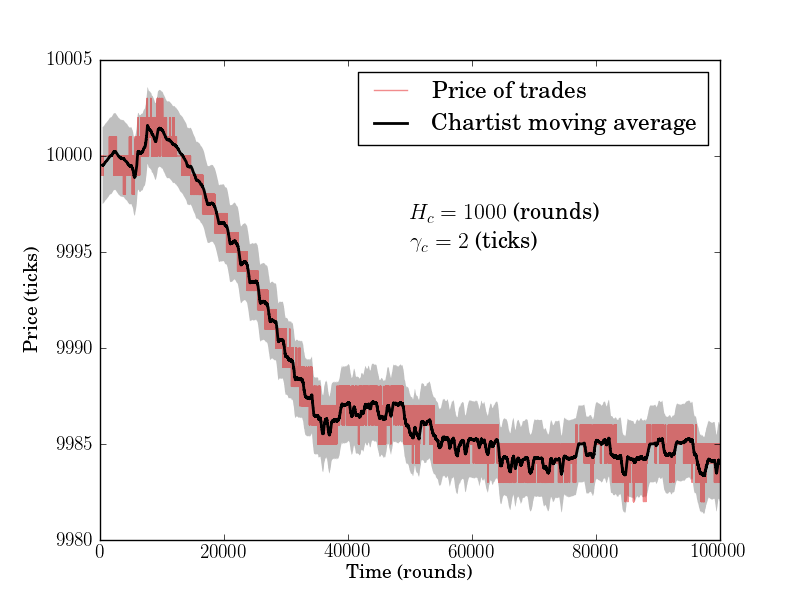
\includegraphics[width=0.7\textwidth]{103_scatter_manual_outlier/d9/f.png}
\caption{Scatter plot of \roundstable, \timetoreachnewfundamental and \stdev}
\label{figure:d9_scatter_fitness_inliers_t_r_logs}
\end{figure}
\begin{figure}
\centering
\includegraphics[width=0.7\textwidth]{103_scatter_manual_outlier/d9/j.png}
\caption{Scatter plot of \overshoot, $\log \roundstable$ and \timetoreachnewfundamental}
\label{figure:d9_scatter_fitness_inliers_t_r_o}
\end{figure}

The line $\timetoreachnewfundamental = \roundstable$ (black dashed line) divides figure \ref{figure:d9_scatter_fitness_inliers_t_r_logs} into region A, (upper left triangle) and region B (lower right triangle). Region A contains the fitness-points of the simulations which are counted as stable \textit{after} they reach the new fundamental, and region B contain those that become stable before. Comparing with 



\begin{enumerate}
\item In figure \ref{figure:d9_scatter_fitness_inliers_t_r_logs}, the density of points is slightly higher around the region defined by $\roundstable = \timetoreachnewfundamental$. This is true both for small and large values of \timetoreachnewfundamental and \roundstable. Furthermore, these points all have small values for $\stdev$. The same points can be identified by looking at figure \ref{figure:d9_scatter_fitness_inliers_a}, where a cloud of points lay around the vertical line $\log \stdev \approx -0.6$.
\begin{enumerate}
	\item The low \stdev also means that the traded price is stable after entering the stability margin. Furthermore, the simulations represented by these same points are among the ones with the most stable traded prices.
	%\item Because of the high correlation between \stdev and \overshoot, simulations belonging to this group have little or no overshoot. 
	\item Since $\timetoreachnewfundamental \approx \roundstable$, the traded does not leave the stability margin once it has entered. This is true for both small and large values of \timetoreachnewfundamental and \roundstable.
\end{enumerate}
\item In figure \ref{figure:d9_scatter_fitness_inliers_t_r_logs} The density seems high in the region defined by the inequalities $0.2 < \timetoreachnewfundamental < 0.3$ and $\roundstable > 0.25$. 
	\begin{enumerate}
	\item Simulations in this group reach the new fundamental quickly (less than $2\cdot 10^4$ rounds after the shock), but then leave the stable region again.
	\item The simulations which take a longer time to become stable also have less stable traded prices (higher values of \stdev)
	\end{enumerate}
\end{enumerate}



\subsubsection{\stdev vs. \timetoreachnewfundamental}
\begin{figure}
\centering
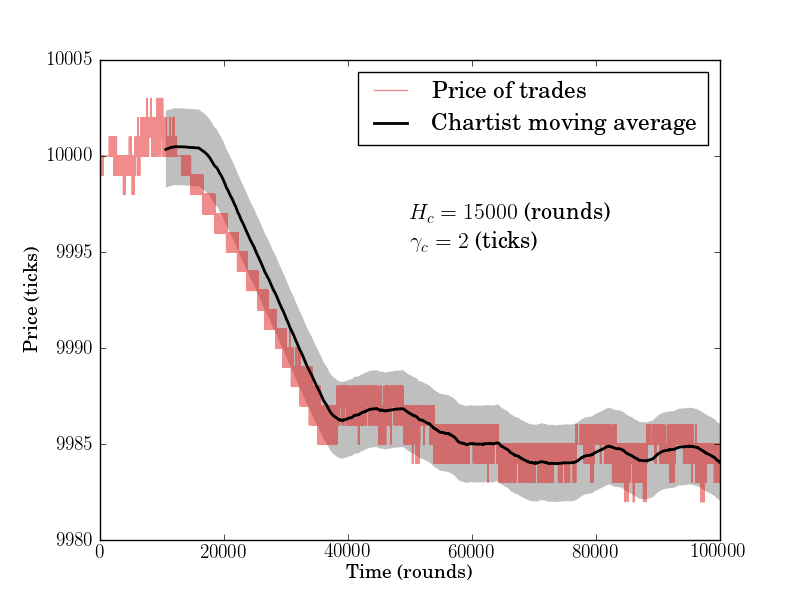
\includegraphics[width=0.7\textwidth]{103_scatter_manual_outlier/d9/h.png}
\caption{Scatter plot of \roundstable, \timetoreachnewfundamental and \stdev}
\label{figure:d9_scatter_fitness_inliers_logs_t_r}
\end{figure}
\begin{figure}
\centering
\includegraphics[width=0.7\textwidth]{103_scatter_manual_outlier/d9/k.png}
\caption{Scatter plot of \roundstable, \timetoreachnewfundamental and \overshoot}
\label{figure:d9_scatter_fitness_inliers_logs_t_o}
\end{figure}

\begin{enumerate}
\item The two large clusters of red points in figure \ref{figure:d9_scatter_fitness_inliers_c} are all the simulations which never became stable during the simulation. The horizontal cluster contain the simulations which responded quickly to the shock by taking only between 10.000 and 20.000 rounds. This cluster contains simulations with both high and low \stdev values, indicating varied behavior.
\item The spike of points on the right side of the cluster are simulations that did become stable, but did so slowly and with no overshoot, as is seen by observing that all the points in the cluster are blue when the color indicated the value of \overshoot as in figure \ref{figure:d9_scatter_fitness_inliers_logs_t_o}.
\end{enumerate}











The next section seeks an answer to the question of whether or not there are model parameters which cause the model to behave in certain ways.
In other words, is it possible to make predictions about the model behavior based of the model parameters?










\subsection{Looking for parameters causing certain behavior}
In order to answer the question posed in the end of the previous section, we can divide the data points into groups based on their fitness values, and then calculate descriptive statistics for the parameters of the points belonging to each group. 

The easiest first step is to do that for the outliers and inliers.


\begin{figure}
\subcaptionbox{}
[0.49\linewidth]{\includegraphics[width=0.5\textwidth]{101_pars_vs_fits/d9/ssmm_latency_mu__vs__round_stable(mean)_scatter.png}}
\subcaptionbox{}
[0.49\linewidth]{\includegraphics[width=0.5\textwidth]{101_pars_vs_fits/d9/ssmm_latency_mu__vs__round_stable(median)_scatter.png}}
\caption{}
\label{figure:d9_parvsfit_ssmm_latency_mu__vs__round_stable(median)_scatter}
\end{figure}



\begin{table}
	 \centering
	 \begin{tabular}{lrrrr}
	\toprule
	{} &  \overshoot > 10 (mean) &  \overshoot > 10 (mean) &  \overshoot > 10 (std) &  \overshoot > 10 (std) \\
	\midrule
	\sclatencymu                &                    73.8 &                    21.2 &                   21.2 &                   13.2 \\
	\sclatencys                 &                     5.2 &                     9.6 &                    9.6 &                    5.7 \\
	\scthinkmu                  &                    64.3 &                    24.3 &                   24.3 &                   13.6 \\
	\scthinks                   &                    11.4 &                    10.2 &                   10.2 &                    5.6 \\
	\sctimehorizonmu            &                  1804.5 &                  2134.1 &                 2134.1 &                 1444.1 \\
	\sctimehorizons             &                  1413.2 &                  1024.0 &                 1024.0 &                  629.2 \\
	\scwaitTimeBetweenTradingmu &                    29.9 &                    23.8 &                   23.8 &                   12.9 \\
	\scwaitTimeBetweenTradings  &                     3.6 &                     9.5 &                    9.5 &                    5.8 \\
	\ssmmlatencymu              &                    46.0 &                    29.9 &                   29.9 &                   14.7 \\
	\ssmmlatencys               &                     4.6 &                     8.8 &                    8.8 &                    5.0 \\
	\ssmmthinkmu                &                    37.6 &                    27.0 &                   27.0 &                   14.2 \\
	\ssmmthinks                 &                     0.9 &                    10.0 &                   10.0 &                    6.0 \\
	\bottomrule
	\end{tabular}
	\label{LABEL}
	\caption{CAPTION}
\end{table}

As manually labeling hundreds of thousands of data points is not really an option, clustering algorithms were used to separate the fitness data into groups with distinct characteristics. 

\subsection{Section summary}


\section{D10}
In the previous section, some weak tendencies 

\begin{figure}
	%issue 15
	\centering
	\subcaptionbox{Evolution of \ssmmlatencymu and \sclatencymu}
	[0.49\linewidth]{\includegraphics[width=0.5\textwidth]{82_generation_plots/d10/latpars_mu.png}}
	\subcaptionbox{Evolution of \ssmmlatencys and \sclatencys}
	[0.49\linewidth]{\includegraphics[width=0.5\textwidth]{82_generation_plots/d10/latpars_s.png}}
	\subcaptionbox{Evolution of \nmm}
	[0.49\linewidth]{\includegraphics[width=0.5\textwidth]{82_generation_plots/d10/nAgents.png}}
	\caption{Evolution of the model parameters in experiment \dten}
	\label{fig:d10_evolution_parameters}
\end{figure}

\begin{figure}
	%issue 15
	\centering
	\subcaptionbox{Evolution of \roundstable}
	[0.49\linewidth]{\includegraphics[width=0.5\textwidth]{82_generation_plots/d10/round_stable.png}}
	\subcaptionbox{Evolution of \timetoreachnewfundamental}
	[0.49\linewidth]{\includegraphics[width=0.5\textwidth]{82_generation_plots/d10/time_to_reach_new_fundamental.png}}
	\subcaptionbox{Evolution of \stdev}
	[0.49\linewidth]{\includegraphics[width=0.5\textwidth]{82_generation_plots/d10/stdev.png}}
	\subcaptionbox{Evolution of \overshoot}
	[0.49\linewidth]{\includegraphics[width=0.5\textwidth]{82_generation_plots/d10/overshoot.png}}
	\caption{Evolution of the four fitness measures in experiment \dten}
	\label{fig:d10_evolution_fitness}
\end{figure}

\begin{figure}
	%issue 15
	\centering
	\subcaptionbox{Correlation between \sclatencymu and \overshoot}
	[0.49\linewidth]{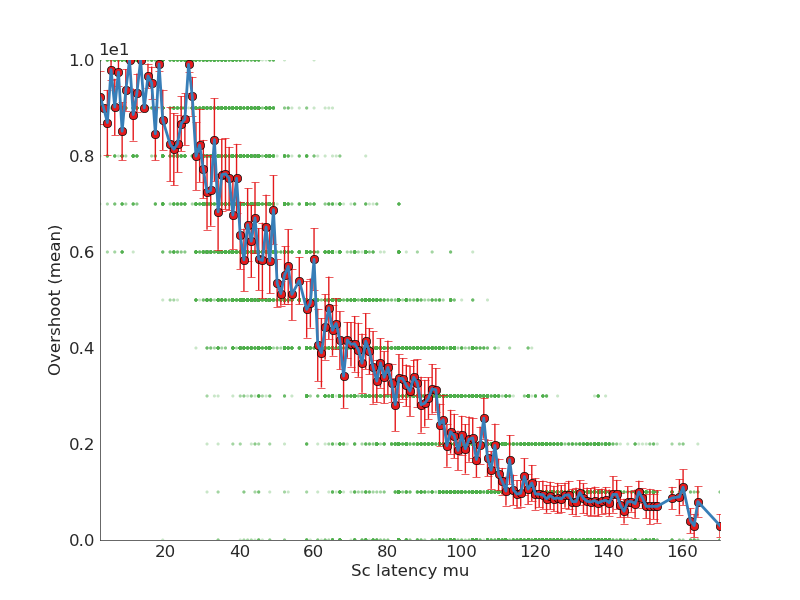
\includegraphics[width=0.5\textwidth]{101_pars_vs_fits/d10/sc_latency_mu__vs__overshoot(mean)_scatter.png}}
	\subcaptionbox{Correlation between \sclatencymu and \roundstable}
	[0.49\linewidth]{\includegraphics[width=0.5\textwidth]{101_pars_vs_fits/d10/sc_latency_mu__vs__round_stable(mean)_scatter.png}}
	\subcaptionbox{Correlation between \sclatencymu and \stdev}
	[0.49\linewidth]{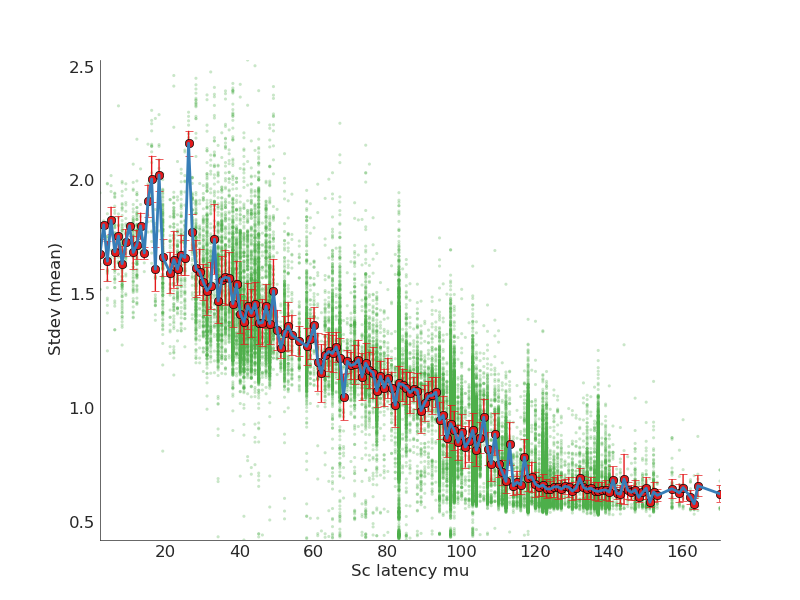
\includegraphics[width=0.5\textwidth]{101_pars_vs_fits/d10/sc_latency_mu__vs__stdev(mean)_scatter.png}}
	\subcaptionbox{Correlation between \sclatencymu and \timetoreachnewfundamental}
	[0.49\linewidth]{\includegraphics[width=0.5\textwidth]{101_pars_vs_fits/d10/sc_latency_mu__vs__time_to_reach_new_fundamental(mean)_scatter.png}}
	
	\caption{Correlation between \sclatencymu and the four fitness measures\dten}
	\label{fig:d10_parvfit_sclatencymu}
\end{figure}

\begin{figure}
	%issue 15
	\centering
	\subcaptionbox{Correlation between \ssmmlatencymu and \overshoot}
	[0.49\linewidth]{\includegraphics[width=0.5\textwidth]{101_pars_vs_fits/d10/ssmm_latency_mu__vs__overshoot(mean)_scatter.png}}
	\subcaptionbox{Correlation between \ssmmlatencymu and \roundstable}
	[0.49\linewidth]{\includegraphics[width=0.5\textwidth]{101_pars_vs_fits/d10/ssmm_latency_mu__vs__round_stable(mean)_scatter.png}}
	\subcaptionbox{Correlation between \ssmmlatencymu and \stdev}
	[0.49\linewidth]{\includegraphics[width=0.5\textwidth]{101_pars_vs_fits/d10/ssmm_latency_mu__vs__stdev(mean)_scatter.png}}
	\subcaptionbox{Correlation between \ssmmlatencymu and \timetoreachnewfundamental}
	[0.49\linewidth]{\includegraphics[width=0.5\textwidth]{101_pars_vs_fits/d10/ssmm_latency_mu__vs__time_to_reach_new_fundamental(mean)_scatter.png}}
	
	\caption{Correlation between \sclatencymu and the four fitness measures\dten}
	\label{fig:d10_parvfit_ssmmlatencymu}
\end{figure}


\begin{figure}
	%issue 15
	\centering
	\subcaptionbox{Correlation between \ssmmnAgents and \overshoot}
	[0.49\linewidth]{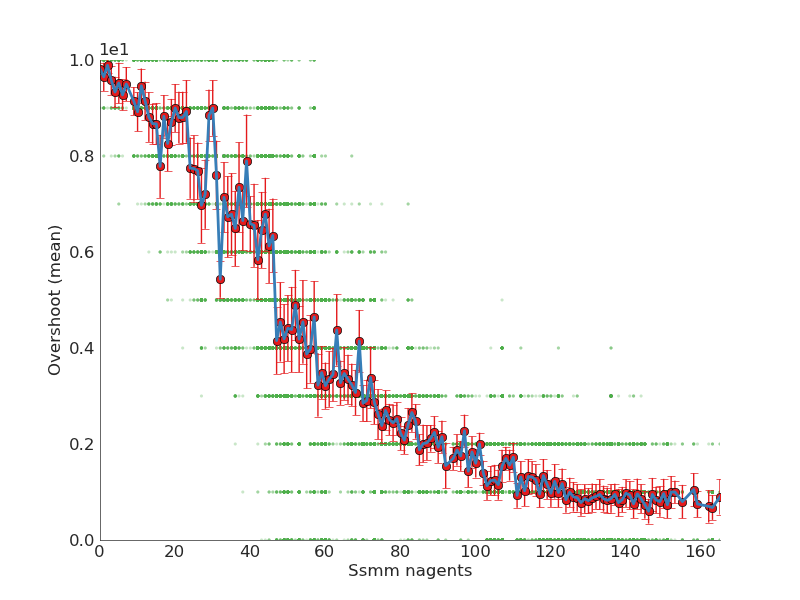
\includegraphics[width=0.5\textwidth]{101_pars_vs_fits/d10/ssmm_nAgents__vs__overshoot(mean)_scatter.png}}
	\subcaptionbox{Correlation between \ssmmnAgents and \roundstable}
	[0.49\linewidth]{\includegraphics[width=0.5\textwidth]{101_pars_vs_fits/d10/ssmm_nAgents__vs__round_stable(mean)_scatter.png}}
	\subcaptionbox{Correlation between \ssmmnAgents and \stdev}
	[0.49\linewidth]{\includegraphics[width=0.5\textwidth]{101_pars_vs_fits/d10/ssmm_nAgents__vs__stdev(mean)_scatter.png}}
	\subcaptionbox{Correlation between \ssmmnAgents and \timetoreachnewfundamental}
	[0.49\linewidth]{\includegraphics[width=0.5\textwidth]{101_pars_vs_fits/d10/ssmm_nAgents__vs__time_to_reach_new_fundamental(mean)_scatter.png}}
	
	\caption{Correlation between \ssmmnAgents and the four fitness measures\dten}
	\label{fig:d10_parvfit_ssmmnAgents}
\end{figure}

\section{D11}


\begin{figure}
	%issue 15
	\centering
	\subcaptionbox{Evolution of \ssmmlatencymu and \sclatencymu}
	[0.49\linewidth]{\includegraphics[width=0.5\textwidth]{82_generation_plots/d11/latpars_mu.png}}
	\subcaptionbox{Evolution of \ssmmlatencys and \sclatencys}
	[0.49\linewidth]{\includegraphics[width=0.5\textwidth]{82_generation_plots/d11/latpars_s.png}}
	\subcaptionbox{Evolution of \nmm}
	[0.49\linewidth]{\includegraphics[width=0.5\textwidth]{82_generation_plots/d11/nAgents.png}}
	\caption{Evolution of the model parameters in experiment \dten}
	\label{fig:d11_evolution_parameters}
\end{figure}

\begin{figure}
	%issue 15
	\centering
	\subcaptionbox{Evolution of \roundstable}
	[0.49\linewidth]{\includegraphics[width=0.5\textwidth]{82_generation_plots/d11/round_stable.png}}
	\subcaptionbox{Evolution of \timetoreachnewfundamental}
	[0.49\linewidth]{\includegraphics[width=0.5\textwidth]{82_generation_plots/d11/time_to_reach_new_fundamental.png}}
	\subcaptionbox{Evolution of \stdev}
	[0.49\linewidth]{\includegraphics[width=0.5\textwidth]{82_generation_plots/d11/stdev.png}}
	\subcaptionbox{Evolution of \overshoot}
	[0.49\linewidth]{\includegraphics[width=0.5\textwidth]{82_generation_plots/d11/overshoot.png}}
	\caption{Evolution of the four fitness measures in experiment \dten}
	\label{fig:d11_evolution_fitness}
\end{figure}

\begin{figure}
	%issue 15
	\centering
	\subcaptionbox{Correlation between \sclatencymu and \overshoot}
	[0.49\linewidth]{\includegraphics[width=0.5\textwidth]{101_pars_vs_fits/d11/sc_latency_mu__vs__overshoot(mean)_scatter.png}}
	\subcaptionbox{Correlation between \sclatencymu and \roundstable}
	[0.49\linewidth]{\includegraphics[width=0.5\textwidth]{101_pars_vs_fits/d11/sc_latency_mu__vs__round_stable(mean)_scatter.png}}
	\subcaptionbox{Correlation between \sclatencymu and \stdev}
	[0.49\linewidth]{\includegraphics[width=0.5\textwidth]{101_pars_vs_fits/d11/sc_latency_mu__vs__stdev(mean)_scatter.png}}
	\subcaptionbox{Correlation between \sclatencymu and \timetoreachnewfundamental}
	[0.49\linewidth]{\includegraphics[width=0.5\textwidth]{101_pars_vs_fits/d11/sc_latency_mu__vs__time_to_reach_new_fundamental(mean)_scatter.png}}
	
	\caption{Correlation between \sclatencymu and the four fitness measures\dten}
	\label{fig:d11_parvfit_sclatencymu}
\end{figure}

\begin{figure}
	%issue 15
	\centering
	\subcaptionbox{Correlation between \ssmmlatencymu and \overshoot}
	[0.49\linewidth]{\includegraphics[width=0.5\textwidth]{101_pars_vs_fits/d11/ssmm_latency_mu__vs__overshoot(mean)_scatter.png}}
	\subcaptionbox{Correlation between \ssmmlatencymu and \roundstable}
	[0.49\linewidth]{\includegraphics[width=0.5\textwidth]{101_pars_vs_fits/d11/ssmm_latency_mu__vs__round_stable(mean)_scatter.png}}
	\subcaptionbox{Correlation between \ssmmlatencymu and \stdev}
	[0.49\linewidth]{\includegraphics[width=0.5\textwidth]{101_pars_vs_fits/d11/ssmm_latency_mu__vs__stdev(mean)_scatter.png}}
	\subcaptionbox{Correlation between \ssmmlatencymu and \timetoreachnewfundamental}
	[0.49\linewidth]{\includegraphics[width=0.5\textwidth]{101_pars_vs_fits/d11/ssmm_latency_mu__vs__time_to_reach_new_fundamental(mean)_scatter.png}}
	
	\caption{Correlation between \sclatencymu{} and the four fitness measures\dten}
	\label{fig:d11_parvfit_ssmmlatencymu}
\end{figure}


\begin{figure}
	%issue 15
	\centering
	\subcaptionbox{Correlation between \nsc{} and \overshoot}
	[0.49\linewidth]{\includegraphics[width=0.5\textwidth]{101_pars_vs_fits/d11/sc_nAgents__vs__overshoot(mean)_scatter.png}}
	\subcaptionbox{Correlation between \nsc{} and \roundstable}
	[0.49\linewidth]{\includegraphics[width=0.5\textwidth]{101_pars_vs_fits/d11/sc_nAgents__vs__round_stable(mean)_scatter.png}}
	\subcaptionbox{Correlation between \nsc{} and \stdev}
	[0.49\linewidth]{\includegraphics[width=0.5\textwidth]{101_pars_vs_fits/d11/sc_nAgents__vs__stdev(mean)_scatter.png}}
	\subcaptionbox{Correlation between \nsc{} and \timetoreachnewfundamental}
	[0.49\linewidth]{\includegraphics[width=0.5\textwidth]{101_pars_vs_fits/d11/sc_nAgents__vs__time_to_reach_new_fundamental(mean)_scatter.png}}
	
	\caption{Correlation between \ssmmnAgents{} and the four fitness measures\dten}
	\label{fig:d11_parvfit_scAgents}
\end{figure}


\section{Hall of fame}
